\hyphenation{аудио-драмах}
\hyphenation{аудио-записях}

\chapter{Аниме: загадочный и поразительный мир японской анимации}

\marginnote[0.0cm]{Сэйю ~--- это японские актёры озвучивания. Сэйю обычно озвучивают роли персонажей в аниме, видеоиграх, фильмах, а также на радио и телевидении, или выступают в роли рассказчика в радиопостановках. Кроме того, голоса сэйю используются в рекламе, голосовых объявлениях, аудиозаписях книг и учебных материалов, а также для переозвучивания. Сэйю могут быть как мужчины, так и женщины; как взрослые, так и дети}

В рамках этой главы исследуется объект Викиданных \wdqName{<<аниме>>}{1107}. С помощью SPARQL-запросов, вычисляемых на объектах типа <<аниме>> в Викиданных, получен список сэйю, упорядоченный по числу озвученных ими аниме, построена гистограмма числа аниме, озвученных одним сэйю, построен граф, связывающий сэйю и озвученные ими аниме, получены оценки трудоспособного возраста сэйю. 

\begin{marginfigure}[0.0cm]
{
	\setlength{\fboxsep}{0pt}%
	\setlength{\fboxrule}{1pt}%
	\fcolorbox{gray}{gray}{\includegraphics{chapter/anime/seyu.jpg}}
}
\caption
[Сэйю]
{
Сэйю Кэндзи Акабанэ озвучивал роль персонажа Sasuke Sarutobi в видеоигре Ikemen Sengoku.\newline
2018 / numan / CC BY-SA 3.0
}
\label{fig:seyu}
\end{marginfigure}

\label{ch:anime}

\section{Экземпляры объекта <<Аниме>>}

Аниме ~--- это японская мультипликация. Она отстоит особняком от анимационных фильмов, создаваемых в других странах. Разумеется, аниме выделяется своим визуальным стилем, однако есть и менее очевидные отличия: так, по сравнению с американской и японской анимацией у аниме значительно шире список жанров ~--- от детских и семейных комедий до драматических историй, которые на Западе обычно изображаются только в фильмах с живыми актёрами\footnote{Аниме VS Мультипликация - CADELTA.RU. \href{https://cadelta.ru/anime/id6119}{https://cadelta.ru/anime/id6119}, 2021.}.

У каждого аниме есть свои актёры озвучивания. В дальнейшем под <<сэйю>> будем понимать японского актёра озвучивания. В японской анимации слова <<актёры озвучивания>> и <<сэйю>> являются синонимами\footnote{Поиск сэйю / Человек. \href{https://
shikimori.one/people/seyu}{https://shikimori.one/people/seyu}, 2021}. Под словом <<тайтл>> (от англ. <<title>>, \emph{название}) обычно понимают конкретное аниме\cite{anime_social}. В общем же смысле слово <<тайтл>> означает понятие, объединяющее различные виды продукции (от кинофильма до романа), созданные на основе конкретного произведения, за которым закреплено строго определённое название\cite{anime_title_def}.

Чтобы работать со списком аниме, о которых есть информация в Викиданных, нам понадобятся объект \wdqName{<<аниме>>}{1107} и свойство \wdProperty{31}{<<экземпляр>>}.

Получим список всех аниме без учёта подклассов (листинг ~\protect\ref{lst:anime}):

\begin{lstlisting}[ language=SPARQL, 
                    caption={\href{https://w.wiki/4ABw}{Список аниме без учёта подклассов}\protect\footnotemark},
                    label=lst:anime,
                    texcl 
                    ]
# List of instances of anime
SELECT ?anime ?animeLabel
WHERE
{
    ?anime wdt:P31 wd:Q1107. # instance of anime
    SERVICE wikibase:label{bd:serviceParam
					     wikibase:language "ru,en,ja"}
}
\end{lstlisting}%
\footnotetext{Получено \num{683} результата в 2017 году и \num{216} результатов в 2021 году. Ссылка на SPARQL-запрос: \href{https://w.wiki/4ABw}{https://w.wiki/4ABw}}

В действительности в Викиданных объектов аниме гораздо больше, но они являются экземплярами не объекта <<аниме>>, а его подклассов, таких как, например, \wdqName{<<аниме-сериал>>}{63952888}. Чтобы получить список жанров аниме и количество аниме, относящихся к этим жанрам, выполним такой запрос (листинг ~\protect\ref{lst:anime_w_subclass}):

\begin{lstlisting}[ language=SPARQL, 
                    caption={\href{https://w.wiki/4ABj}{Список жанров аниме и количество аниме, относящихся к этим жанрам}\protect\footnotemark},
                    label=lst:anime_w_subclass,
                    texcl 
                    ]
# Select anime and its subclasses with number of titles
# corresponding to these subclasses
SELECT ?subAnime ?subAnimeLabel (COUNT(?subAnimeInst) AS ?count)
WHERE {
  ?subAnime wdt:P279* wd:Q1107.       # select anime subclass list
  ?subAnimeInst wdt:P31 ?subAnime # link titles and subclasses
    SERVICE wikibase:label{bd:serviceParam
					     wikibase:language "ru,en,ja"}
}
GROUP BY ?subAnime ?subAnimeLabel
ORDER BY DESC(?count)
\end{lstlisting}%
\footnotetext{Получено \num{11} результатов в 2021 году. Ссылка на SPARQL-запрос: \href{https://w.wiki/4ABj}{https://w.wiki/4ABj}}

Полученная классификация аниме по жанрам не идеальна, так как есть большое смещение в сторону аниме-сериалов: из 4757 тайтлов 2917 отнесены к жанру <<аниме-сериал>> (61,3 \%); вероятно, классификация жанров аниме в Викиданных требует дальнейшего уточнения. Также в подклассы попали понятия, относящиеся не к общей классификации, а к отдельным аниме, например, \href{https://w.wiki/4L5p}{<<Евангелион>>}.

\begin{marginfigure}[0.0cm]
{
	\setlength{\fboxsep}{0pt}%
	\setlength{\fboxrule}{1pt}%
	\fcolorbox{gray}{gray}{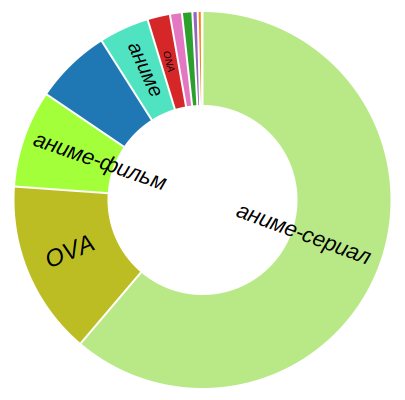
\includegraphics{chapter/anime/anime-subclasses-sunburst-diagram-2021.png}}
}
\caption
[Pie chart]
{
Круговая диаграмма (pie chart) жанров аниме, визуализированный с помощью сервиса \href{https://app.rawgraphs.io}{https://app.rawgraphs.io}.\newline
}
\label{fig:anime_piechart}
\end{marginfigure}

Получим список всех аниме, включая тайтлы, относящиеся к жанрам аниме (листинг ~\protect\ref{lst:all_anime_list}):

\begin{lstlisting}[ language=SPARQL, 
                    caption={\href{https://w.wiki/49zY}{Список всех аниме в Викиданных}\protect\footnotemark},
                    label=lst:all_anime_list,
                    texcl 
                    ]
# List of instances of anime and subclasses of anime
SELECT ?anime ?animeLabel
WHERE
{
    ?anime wdt:P31/wdt:P279* wd:Q1107. # instance of anime/subclass
    SERVICE wikibase:label{bd:serviceParam
					     wikibase:language "ru,en,ja"}
}
\end{lstlisting}%
\footnotetext{Получено \num{683} результата в 2017 году и \num{4756} результатов в 2021 году. Ссылка на SPARQL-запрос: \href{https://w.wiki/49zY}{https://w.wiki/49zY}}

Аниме, о которых есть наиболее полная информация на Викиданных ~--- это \wdqName{Гуррен-Лаганн}{4277}, \wdqName{Space Battleship Yamato}{4292}, \wdqName{Project A-ko}{4316}. Аниме с малоинформативными записями на Викиданных оказались \wdqName{Doraemon}{711311}, \wdqName{The Animal Conference on the Environment}{97195557}, \wdqName{Assassins Pride}{96737300}.

Среди всех аниме-тайтлов в Викиданных больше всего свойств по данным сервиса ProWD\cite{anime_prowd} у \wdqName{Fullmetal Alchemist: The Sacred Star of Milos}{1004318} (24 свойства).

\subsection{Список сэйю, упорядоченный по числу озвученных ими аниме}

Разумеется, в большинстве аниме участвует не один, а множество персонажей. Соответственно, разных персонажей озвучивают разные сэйю. Большинство сэйю озвучили за свою карьеру несколько тайтлов, а многие ~--- несколько десятков тайтлов. Талантливых сэйю приглашают озвучивать сразу несколько персонажей в одном аниме. Одним из самых популярных сэйю является \href{https://w.wiki/4L5q}{Хироси Камия}, имеющий множество наград и озвучивший более 180 аниме. Самым известным аниме с его участием является \href{https://w.wiki/4L5r}{<<Атака титанов>>}, где он озвучил одного из главных персонажей ~--- капитана Леви.

Построим упорядоченный список сэйю по числу озвученных ими аниме (листинг ~\protect\ref{lst:seiyu_titles_sorted}): 

\footnotetext{Получено \num{148} результатов в 2017 году и \num{2684} результата в 2021 году. Ссылка на SPARQL-запрос: \href{https://w.wiki/49zz}{https://w.wiki/49zz}}
\begin{lstlisting}[ language=SPARQL, 
                    caption={\href{https://w.wiki/49zz}{Упорядоченный список сэйю по числу озвученных ими аниме}\protect\footnotemark},
                    label=lst:seiyu_titles_sorted,
                    texcl 
                    ]
# Ordered list of seiyu according to the number of anime
# where they took part in
SELECT ?seiyu (SAMPLE(?label) AS ?seiyuLabel) (COUNT(?anime) AS ?count)
WHERE
{
  ?anime wdt:P31/wdt:P279* wd:Q1107;	 # instance of anime/subclass
         wdt:P725 ?seiyu. 	             # instance of seiyu
  ?seiyu rdfs:label ?label	             # subclass of label
    SERVICE wikibase:label{bd:serviceParam
					     wikibase:language "ru,en,ja"}
}
GROUP BY ?seiyu		    # group by seiyu 
ORDER BY DESC(?count)	# order by count of voiced anime
\end{lstlisting}%

\subsection{График по числу сэйю, озвучивших одно и более аниме}

Было бы интересно построить график (линейную диаграмму) сэйю, озвучивших аниме. Чем больше аниме озвучил сэйю, тем правее на диаграмме он будет находиться. Сделать это можно с помощью скрипта ~\protect\ref{lst:seiyu_titles_graph}.

\begin{fullwidth}
\lstset{numbers=left, firstnumber=1, frame=single}
\begin{lstlisting}[ language=SPARQL, 
                    caption={\href{https://w.wiki/4JvT}{Построение графика по числу сэйю, озвучивших одно и более аниме}\protect\footnotemark},
                    label=lst:seiyu_titles_graph,
                    texcl 
                    ]
# Graph of the number of voice actings of different seiyu
#defaultView:LineChart
SELECT ?seiyuRoles (COUNT(?seiyuRoles) AS ?quantity) WHERE {
  FILTER(?seiyuRoles < 71) # limit the output as there are few seiyu that act in more than 71 anime
  {
     SELECT (COUNT(?seiyu) AS ?seiyuRoles) WHERE {            # count quantity of voice acting by one seiyu
       ?anime wdt:P31/wdt:P279* wd:Q1107;                     # instance of anime and its subclasses
              wdt:P725 ?seiyu.                                # instance of seiyu
       SERVICE wikibase:label { bd:serviceParam wikibase:language "ru,en,ja"}
     }
     GROUP BY ?anime              # group list by number of voiced anime
     ORDER BY DESC(?seiyuRoles)   # order by voice acting quantity (descending)
  }
}
GROUP BY ?seiyuRoles
ORDER BY DESC(?seiyuRoles)  # grouping and sorting seiyu by number of voice actings
\end{lstlisting}%
\footnotetext{Получено \num{13} результатов в 2017 году и \num{58} результатов в 2021 году. Ссылка на SPARQL-запрос: \href{https://w.wiki/4JvT}{https://w.wiki/4JvT}}
\lstset{numbers=none}
\end{fullwidth}

Очевидно, что чем большее количество аниме берётся в расчёт, тем меньшее количество сэйю участвует в озвучке (рис. ~\ref{fig:Seiyu_num_chart_2021_ru}). Многие сэйю, как показано на диаграмме, озвучили только одно аниме — на графике их оказалось 254. Это может быть связано с неполнотой Викиданных. 

\begin{figure*}[h]

    \setlength{\fboxsep}{0pt}%
    \setlength{\fboxrule}{1pt}%
    \fcolorbox{gray}{gray}{\includegraphics[width=\linewidth]{./chapter/anime/Seiyu_chart_2021_ru.png}}
	\caption[График числа ролей, озвученных различными сэйю, 2021.]{График числа ролей, озвученных различными сэйю, 2021. График построен на основе данных, полученных с помощью запроса~\protect\ref{lst:seiyu_titles_graph}.}%
    \label{fig:Seiyu_num_chart_2021_ru}%
\end{figure*} 

\newpage

Аналогичный график можно построить с помощью \href{https://app.rawgraphs.io}{https://app.rawgraphs.io} (рис. ~\ref{fig:anime_seiyu_rawgraphs}).

\begin{figure*}[h]

    \setlength{\fboxsep}{0pt}%
    \setlength{\fboxrule}{1pt}%
    \fcolorbox{gray}{gray}{\includegraphics[width=\linewidth]{./chapter/anime/anime-seiyu-rawgraphs-2021.png}}
	\caption[График числа ролей, озвученных различными сэйю, построенный с помощью сервиса Rawgraphs, 2021.]{График числа ролей, озвученных различными сэйю, построенный с помощью сервиса Rawgraphs, 2021. График построена на основе данных, полученных с помощью запроса~\protect\ref{lst:seiyu_titles_graph}.}%
    \label{fig:anime_seiyu_rawgraphs}%
\end{figure*} 

\subsection{Граф, связывающий сэйю и озвученные ими аниме}

Итак, многие сэйю за свою карьеру успевают озвучить несколько аниме. Чтобы нагляднее показать эту взаимосвязь, построим граф, связывающий сэйю и озвученные ими аниме с помощью скрипта ~\protect\ref{lst:seiyu_graph}. Фрагмент итогового графа представлен на рис. ~\ref{fig:Seiyu_graph_2021_ru}. 

\lstset{numbers=left, firstnumber=1, frame=single}
\begin{lstlisting}[ language=SPARQL, 
                    caption={\href{https://w.wiki/4HFt}{Построение графа, связывающего сэйю и озвученные ими аниме}\protect\footnotemark},
                    label=lst:seiyu_graph,
                    texcl 
                    ]
# Graph of seiyu with more than one anime
#defaultView:Graph
SELECT DISTINCT ?item ?itemLabel ?rgb ?link
WHERE
{ # voice actors (seiyu) with more than one anime
  VALUES ?toggle { true false }
  VALUES ?seiyu { wd:Q6381410 wd:Q1347031 wd:Q1207010 
           wd:Q233902  wd:Q1323728 wd:Q2440809 
           wd:Q355173  wd:Q957795  wd:Q50033}
  ?anime  wdt:P31/wdt:P279* wd:Q1107; # instance of anime/subclass
           wdt:P725 ?seiyu;            # seiyu who voiced this anime 
  SERVICE wikibase:label{bd:serviceParam
					   wikibase:language "ru,en,ja"}
  BIND(IF(?toggle,?anime,?seiyu) AS ?item).
  BIND(IF(?toggle,?animeLabel,?seiyuLabel) AS ?itemLabel).
  BIND(IF(?toggle,"FFFFFF","7FFF00") AS ?rgb).
  BIND(IF(?toggle,"",?anime) AS ?link).
}
\end{lstlisting}%
\footnotetext{Получено \num{826} результатов в 2017 году и \num{494} результата в 2021 году. Ссылка на SPARQL-запрос: \href{https://w.wiki/4HFt}{https://w.wiki/4HFt}}
\lstset{numbers=none}

В переменную \emph{?seiyu} (7-9 строки) записан массив объектов Викиданных, соответствующих некоторым известным сэйю ~--- \wdqName{Кадзуэ Комия}{6381410} и другим.

Конструкция \emph{BIND(IF(?toggle, ?anime1, ?seiyu2))} в строке 14 позволяет определить тип вершины графа: если \emph{?toggle} принимает значение true, то вершина графа соответствует аниме, иначе ~--- сэйю. Аналогично в строках 15 и 16 определяется тип текстовой метки для вершины и цвет вершины.

\newpage
\begin{fullwidth}
\begin{figure*}[h]
	\includegraphics[width=\textwidth]{./chapter/anime/Seiyu_graph_2021_ru.jpg}
	\caption[Фрагмент графа, связывающего сэйю и озвученные ими аниме, 2021.]{Фрагмент графа, связывающего сэйю и озвученные ими аниме, 2021. Граф построен на основе данных, полученных с помощью запроса~\protect\ref{lst:seiyu_graph}.}%
      \label{fig:Seiyu_graph_2021_ru}%
\end{figure*} 
\end{fullwidth}

\section{Полнота Викиданных}

Список тайтлов в \href{https://w.wiki/4JVE}{Русской Википедии}\footnote{Проект:Аниме и манга/Списки/Список аниме. \href{https://w.wiki/4JVE}{https://w.wiki/4JVE}, 2021} содержит \num{1638} аниме. Также можно посмотреть \href{https://w.wiki/4JVH}{телевизионные показы аниме в России по годам}\footnote{Проект:Аниме и манга/Телевизионные показы аниме в России по годам. \href{https://w.wiki/4JVH}{https://w.wiki/4JVH}, 2021}.

На сайте \href{https://shikimori.one/}{Shikimori}\cite{shikimori} в списке аниме \num{801} страница по \num{20} наименований. Нетрудно подсчитать, что на сайте есть информация о \num{16020} тайтлах, в то время как в Викиданных объектов, описывающих аниме, всего \num{4756} (см. листинг ~\protect\ref{lst:all_anime_list}). К тому же, стоит учитывать, что скорость выхода новых аниме довольно велика\footnote{Упражнение: с помощью SPARQL подсчитайте, сколько аниме вышло за прошлый год.}. Из этого можно сделать вывод, что Викиданные крайне неполно отражают данные (есть информация только о \num{29.6}\% аниме). То же самое касается и жанров: в \href{https://shikimori.one/animes}{разделе поиска Shikimori}\footnote{Лучшие аниме. \href{https://shikimori.one/animes}{https://shikimori.one/animes}, 2021} доступны \num{42} жанра аниме, в то время как Викиданные содержат информацию только о \num{17}\footnote{Список жанров (категорий) аниме, зарегистрированных в Викиданных, можно посмотреть по ссылке \href{https://en.wikipedia.org/wiki/Category:Lists\_of_anime\_by\_genre}{https://en.wikipedia.org/wiki/Category:Lists\_of\_anime\_by\_genre}}.

Возможно, приведённые ниже статьи и сайты не будут являться \href{https://w.wiki/3u9v}{АИ}\footnote{Авторитетный источник (АИ) ~--- это ресурс, который владеет информацией, в компетентности и актуальности которой не может быть никаких сомнений. См. \href{https://w.wiki/3u9v}{https://w.wiki/3u9v}}, но с их помощью можно проанализировать информацию об имеющихся аниме и сделать дополнительные выводы о неполноте Викиданных.

\begin{itemize}
	\item На сайте \href{http://online.anidub.best/}{AniDub}\footnote{АниДаб. \href{http://online.anidub.best/}{http://online.anidub.best/}, 2021} приведён список из \num{5756} аниме.
	\item На сайте \href{http://animespirit.tv/}{AnimeSpirit}\footnote{AnimeSpirit. \href{http://animespirit.tv/}{http://animespirit.tv/}, 2021} приведён список из \num{1968} аниме.
	\item На сайте \href{http://animeland.su/}{AnimeLand}\footnote{AnimeLand. \href{http://animeland.su/}{http://animeland.su/}, 2021} приведён список из \num{4795} аниме.
	\item На сайте \href{https://anivost.org/}{Anivost}\footnote{Anivost. \href{https://anivost.org/}{https://anivost.org/}, 2021} приведён список из \num{420} аниме.
\end{itemize}

Можно сделать вывод, что различные сайты имеют разную информацию об имеющихся аниме. Какие-то сайты появились позже, какие-то раньше, поэтому количество аниме на них может разниться, причём довольно серьёзно. Если упорядочить все приведённые сайты, данные Русской Википедии, Английской Википедии и Викиданные по количеству аниме, то Викиданные окажутся не на последнем месте, но, например, сайту \href{https://shikimori.one/}{Shikimori}\cite{shikimori} они уступают почти в 4 раза.

Вспомним запрос ~\protect\ref{lst:seiyu_titles_sorted}, в котором говорилось о \num{2684} сэйю на Викиданных. Дело в том, что поиск производился только по актёрам озвучивания, связанным с аниме, поэтому результат оказался таким скромным. Если запросить информацию о всех актёрах озвучивания (то есть убрать ограничение на категорию аниме), то результат может измениться (листинг ~\protect\ref{lst:voice_actors_list}). 

\begin{lstlisting}[ language=SPARQL, 
                    caption={\href{https://w.wiki/4KQY}{Получение списка актёров озвучки и числа озвученных ими проектов}\protect\footnotemark},
                    label=lst:voice_actors_list,
                    texcl 
                    ]
# Ordered list of actors according to the quantity of projects
# voiced by them
SELECT ?actor (SAMPLE(?label) AS ?actorLabel) (COUNT(?media) AS ?count)
WHERE
{
  ?media wdt:P725 ?actor.	 # instance of voice actor
  ?actor rdfs:label ?label	 # subclass of label
  SERVICE wikibase:label { bd:serviceParam
                           wikibase:language "ru,en,ja" }
}
GROUP BY ?actor		    # group by actor
ORDER BY DESC(?count)	# order by number of voiced projects 
\end{lstlisting}%
\footnotetext{Получено \num{3965} результатов в 2017 году и \num{14252} результата в 2021 году. Ссылка на SPARQL-запрос: \href{https://w.wiki/4KQY}{https://w.wiki/4KQY}}

Значительный прирост числа результатов относительно вышеупомянутого запроса говорит о том, что сэйю могут озвучивать не только аниме, но и другие проекты, и это нужно учитывать при формировании запросов.

\section{Указана ли дата публикации у аниме?}

Каждый любитель японской анимации желает знать, в каком году вышло его любимое аниме. Викиданные располагают этой информацией не в полной мере. Напишем скрипт, который бы показывал количество аниме с незаполненным полем ''publication date'' (дата публикации) (листинг ~\protect\ref{lst:anime_no_pub_date}). 

\begin{lstlisting}[ language=SPARQL, 
                    caption={\href{https://w.wiki/4Hcz}{Получение списка аниме, у которых на Викиданных не указана дата выхода}\protect\footnotemark},
                    label=lst:anime_no_pub_date,
                    texcl 
                    ]
# List of anime the release date of which is empty
SELECT ?anime ?animeLabel
WHERE
{
    ?anime wdt:P31/wdt:P279* wd:Q1107;                # instance of anime
    FILTER NOT EXISTS { ?anime wdt:P577 [] }
    SERVICE wikibase:label{bd:serviceParam
					     wikibase:language "ru,en,ja"}
}
\end{lstlisting}%
\footnotetext{Получено \num{237} результатов в 2017 году и \num{2940} результатов в 2021 году. Ссылка на SPARQL-запрос: \href{https://w.wiki/4Hcz}{https://w.wiki/4Hcz}}

На 2021 год из \num{4756} аниме на Викиданных (см. листинг ~\protect\ref{lst:all_anime_list}) у \num{2940}, а это \num{62}\%, не указана дата выхода. В 2017 году из \num{683} аниме на Викиданных только \num{237} (то есть \num{35}\%) не имели указанной даты выхода. Похоже, что, к сожалению, увеличение количества информации не всегда сопровождается сохранением её качества\footnote{Упражнение: напишите скрипт для вычисления доли аниме, у которых не указана дата публикации, относительно всех аниме на Викиданных. Сравните эту долю с долей за 2021 год (\num{62}\%) и сделайте вывод об изменении качества Викиданных.}.

\section{Анализ возраста, в котором сэйю озвучивают аниме}

Как и в любой другой профессии, у актёра озвучки есть возраст, когда он находится в <<расцвете сил>> и может озвучить множество аниме. Использование SPARQL и внешних инструментов для анализа данных, таких как язык программирования Python\footnote{Язык Python ~--- это интерпретируемый язык программирования, благодаря своей гибкости используемый для разнообразных задач. Его можно применять в том числе и для работы с Викиданными: например, в разделе ~\ref{ch:bots} (с.~\pageref{ch:bots}) описан процесс создания программных ботов для Викиданных.}, может позволить оценить такой возраст на основе информации из Викиданных.

Чтобы получить исходные данные для исследования, необходимо выполнить три SPARQL-скрипта и экспортировать результаты их выполнения в формате .csv\footnote{CSV (comma-separated values) ~--- это формат представления табличных данных, в котором таблица хранится в виде последовательности строк текста. Эти строки содержат значения полей таблицы, разделённые запятыми.}.

Получить список всех зарегистрированных в Викиданных сэйю и их дат рождения можно двумя способами (листинги  ~\protect\ref{lst:seiyu_bd_w_service} и  ~\protect\ref{lst:seiyu_bd_w_rdfs}): 

\begin{lstlisting}[ language=SPARQL, 
                    caption={\href{https://w.wiki/4FPq}{Получение дат рождения сэйю (вариант 1)}\protect\footnotemark},
                    label=lst:seiyu_bd_w_service,
                    texcl 
                    ]
# Get list of all seiyu objects, their names and birth dates
SELECT ?seiyu ?seiyuLabel ?bDate WHERE {
  ?anime (wdt:P31/(wdt:P279*)) wd:Q1107;
    wdt:P725 ?seiyu.       # seiyu is anime voice actors
  ?seiyu wdt:P569 ?bDate.  #       has a birthday
    SERVICE wikibase:label{bd:serviceParam
					     wikibase:language "ru,en,ja"}
}
GROUP BY ?seiyu ?seiyuLabel ?bDate
\end{lstlisting}%
\footnotetext{Получено \num{2515} результатов в 2021 году. Ссылка на SPARQL-запрос: \href{https://w.wiki/4FPq}{https://w.wiki/4FPq}}

\begin{lstlisting}[ language=SPARQL, 
                    caption={\href{https://w.wiki/4FPn}{Получение дат рождения сэйю (вариант 2)}\protect\footnotemark},
                    label=lst:seiyu_bd_w_rdfs,
                    texcl 
                    ]
# Get list of all seiyu objects, their names and birth dates
SELECT ?seiyu (SAMPLE(?seiyu) AS ?seiyuLabel) ?bDate WHERE {
  ?anime (wdt:P31/(wdt:P279*)) wd:Q1107;
    wdt:P725 ?seiyu.       # seiyu is anime voice actors
  ?seiyu wdt:P569 ?bDate.  #       has a birthday 
  ?seiyu rdfs:label ?label.
}
GROUP BY ?seiyu ?bDate
\end{lstlisting}%
\footnotetext{Получено \num{2515} результатов в 2021 году. Ссылка на SPARQL-запрос: \href{https://w.wiki/4FPn}{https://w.wiki/4FPn}}

Различия между скриптами (листинги  ~\protect\ref{lst:seiyu_bd_w_service} и  ~\protect\ref{lst:seiyu_bd_w_rdfs}) заключаются в том, что:

\begin{itemize}
    \item метка (имя) сэйю в первом случае получается с помощью переменной \emph{?seiyuLabel} (в таком случае нужно указать команду \emph{SERVICE} для установки языков, на котором будут возвращены имена), а во втором ~--- с помощью конструкции \emph{rdfs:label};
    \item в первом варианте скрипта необходимо указывать \emph{?seiyuLabel} как параметр \emph{GROUP BY}, чтобы связать объекты сэйю и их метки.
\end{itemize}

Получим список всех зарегистрированных в Викиданных аниме и дат их выхода (листинг ~\protect\ref{lst:all_anime_releases}).\footnote{Упражнение: визуализируйте результаты работы скрипта ~\protect\ref{lst:all_anime_releases}. Можете усложнить задачу ~--- например, добавить на график даты окончания показа сериалов.} 

\begin{lstlisting}[ language=SPARQL, 
                    caption={\href{https://w.wiki/4ENc}{Получение дат выхода аниме}\protect\footnotemark},
                    label=lst:all_anime_releases,
                    texcl 
                    ]
# Get all anime objects, their names and release dates
SELECT ?anime ?animeLabel ?animePubDate ?animeSeriesStartDate
WHERE {
  ?anime (wdt:P31/(wdt:P279*)) wd:Q1107.               # object of anime/subclass
  OPTIONAL { ?anime wdt:P577 ?animePubDate. }          # release date of a movie
  OPTIONAL { ?anime wdt:P580
					?animeSeriesStartDate. }  # start date of a series
    SERVICE wikibase:label{bd:serviceParam
					     		wikibase:language "ru,en,ja"}
}
\end{lstlisting}%
\footnotetext{Получено \num{5264} результатов в 2021 году. Ссылка на SPARQL-запрос: \href{https://w.wiki/4ENc}{https://w.wiki/4ENc}}

Обратите внимание, что скрипт (листинг ~\protect\ref{lst:all_anime_releases}) получает не только  \wdProperty{577}{даты выхода полнометражных аниме}, но и \wdProperty{580}{даты начала показа сериалов}. 

Получение ссылок между объектами сэйю и аниме, которые они озвучивали (листинг ~\protect\ref{lst:link_anime_seiyu}): 

\begin{lstlisting}[ language=SPARQL, 
                    caption={\href{https://w.wiki/4ELh}{Получение ссылок между сэйю и аниме}\protect\footnotemark},
                    label=lst:link_anime_seiyu,
                    texcl 
                    ]
# List of links between seiyu and anime where they are involved in
SELECT DISTINCT ?item ?itemLabel ?link ?itemType
WHERE
{
  VALUES ?toggle { true false }
  ?anime  wdt:P31/wdt:P279* wd:Q1107; # instance of anime/subclass
          wdt:P725 ?seiyu.            # list seiyu who acted in this anime
  
  BIND(IF(?toggle,?anime,?seiyu) AS ?item).   # anime/seiyu link
  BIND(IF(?toggle,?animeLabel,?seiyuLabel)
					AS ?itemLabel).  # anime/seiyu labels link
  BIND(IF(?toggle,?seiyu,?anime) AS ?link).   # seiyu/anime link
  BIND(IF(?toggle,?seiyu,"seiyu")
							AS ?itemType).
    SERVICE wikibase:label{bd:serviceParam
					     		wikibase:language "ru,en,ja"}
}
\end{lstlisting}%
\footnotetext{Получено \num{27092} результата в 2021 году. Ссылка на SPARQL-запрос: \href{https://w.wiki/4ELh}{https://w.wiki/4ELh}}

Результат анализа удобно представить в виде гистограммы. Для её построения можно воспользоваться средствами таких библиотек для Python, как \href{https://ru.wikipedia.org/wiki/Pandas}{Pandas}\footnote{pandas. \href{https://ru.wikipedia.org/wiki/Pandas}{https://ru.wikipedia.org/wiki/Pandas}, 2021} для обработки табличных данных и \href{https://ru.wikipedia.org/wiki/Matplotlib}{Matplotlib}\footnote{Matplotlib. \href{https://ru.wikipedia.org/wiki/Matplotlib}{https://ru.wikipedia.org/wiki/Matplotlib}, 2021} для непосредственно построения графиков. Код скрипта, создающего гистограмму, опубликован на сервисе \href{https://github.com/componavt/wd_book/blob/master/programming_tasks/seiyu_age/age_act_hist.ipynb}{GitHub}\footnote{Ссылка на скрипт: \href{https://clck.ru/Yc5Pg}{https://clck.ru/Yc5Pg}}.

В результате получим гистограмму, по оси абсцисс которой отложен возраст в годах, а по оси ординат ~--- суммарное количество ролей, озвученных всеми сэйю такого возраста. Получившаяся гистограмма представлена на рис. ~\ref{fig:Seiyu_age_hist_RU}. 

\begin{figure*}[h]

    \setlength{\fboxsep}{0pt}%
    \setlength{\fboxrule}{1pt}%
    \fcolorbox{gray}{gray}{\includegraphics[width=\linewidth]{./chapter/anime/Seiyu_age_hist_RU.png}}
	\caption[Гистограмма, которая отображает число аниме, озвученное сэйю разных возрастов, 2021.]{Гистограмма, которая показывает число аниме, озвученных различными сэйю, 2021. Гистограмма построена на основе данных, полученных с помощью запроса ~\protect\ref{lst:link_anime_seiyu}.}%
    \label{fig:Seiyu_age_hist_RU}%
\end{figure*} 
 	
Отметим следующий забавный факт: в Викиданных нашлись случаи, когда сэйю родился(-ась) позже, когда вышло аниме с его (её) участием. В данных есть забавные моменты, когда сэйю родился(-ась) позже, когда вышло аниме с его (её) участием. Вероятно, это связано с отсутствием информации в Викиданных о втором сезоне/перезапуске аниме. Например, на 2021 год такая ситуация наблюдается для аниме \wdqName{Sazae-san}{11304591} и сэйю \wdqName{Нобунага Симадзаки}{5968283}.

\section{Упражнения}

\begin{enumerate}
    \item Вывести 10 аниме, выпущенных в текущем году.
    \item Вывести 5 аниме, в которых задействовано самое большое число сэйю.
    \item Построить пузырьковую диаграмму (BubbleChart) распределения аниме по жанрам (сколько аниме в каждом жанре), воспользовавшись свойством \wdProperty{279}{<<подкласс>> (P279)}.
    \item Отметить на карте места рождения сэйю.
    \item Построить гистограмму или пузырьковую диаграмму национальностей сэйю.
    \item Построить гистограмму количества вышедших аниме по годам или количества сэйю по годам рождения.
    \item Построить гистограммы, аналогичные рисунку ~\ref{fig:Seiyu_age_hist_RU}, но с учётом пола сэйю (одну для мужчин, другую для женщин).
\end{enumerate}